\documentclass[10pt,twocolumn,letterpaper]{article}

\usepackage{statcourse}
\usepackage{times}
\usepackage{epsfig}
\usepackage{graphicx}
\usepackage{amsmath}
\usepackage{amssymb}
\usepackage{graphicx}
\graphicspath{ {./figures/} }

% Include other packages here, before hyperref.

% If you comment hyperref and then uncomment it, you should delete
% egpaper.aux before re-running latex.  (Or just hit 'q' on the first latex
% run, let it finish, and you should be clear).
\usepackage[breaklinks=true,bookmarks=false]{hyperref}


\statcoursefinalcopy


\setcounter{page}{1}
\begin{document}


%%%%%%%%%%%%%%%%%%%%%%%%%%%%%%%%%%%%%%%%%%%%%%%%%%%%%%%%%%%%%%%
% DO NOT EDIT ANYTHING ABOVE THIS LINE
% EXCEPT IF YOU LIKE TO USE ADDITIONAL PACKAGES
%%%%%%%%%%%%%%%%%%%%%%%%%%%%%%%%%%%%%%%%%%%%%%%%%%%%%%%%%%%%%%%



%%%%%%%%% TITLE
\title{ Twitter Posts Political Ideology Classification }

\author{Han Cao \\
{\tt\small hcao29@wisc.edu }
\and
Siyi He \\
{\tt\small she83@wisc.edu }
\and
Qiwen Zeng\\
{\tt\small qzeng36@wisc.edu}
}
\maketitle

\section{Introduction}
According to several articles released recently\cite{parks_2020}, Internet companies can potentially have the power of manipulating the political ideologies of the public to achieve the goals of private parties. We want to develop a tool that can help us understand the public opinions of political ideologies on social media. 

Machine learning can be used to achieve such a purpose. Natural language processing has been significantly developed in the past decades. There already exist applications using machine learning to perform analysis on the sentiment of twitters.

We propose to use machine learning techniques to identify political ideologies behind social media texts. Given the context of 2020 presidential election is happening, we want to classify whether a text implies Democratic or Republican ideas. 

Twitter is one of the most influential social platforms. Many politicians or political organizations use Twitter to broadcast to their audiences. Thus we decide to train our model using labeled twitter posts. 

The goal of this project is to train one or several machine learning models to classify political ideologies, specifically Democratic and Republican ideas, using machine learning model trained with Twitter posts. 

\section{Related Work}
In work from 2009\cite{yu_kaufmann_diermeier}, Yu, Kaufmann, diermeier established a pipeline for developing ideology classifier for political speeches. We would like to try some suggestions from this paper.

Here is another project\cite{bhand_robinson_sathi}, also try to classify political ideologies but with political speeches. In the paper, the authors discussed the performance of different models. We will borrow some experiences from this research to select models that are suitable for our problem.

\section{Motivation}
\subsection{Related Event}
The main motivation for researching this topic comes from the ongoing presidential election. We are curious about the trends of supporting Democrat or Republican on popular social media. By developing such a tool, we can monitor public opinions on social media. On the one hand, by doing so, we can potentially try to form a trend of public opinion shifting of political ideologies. By drawing connections with key events, we can investigate the impact of such events on public opinions. On the other hand, by using such a tool, we can also classify the user's political affiliation based on the text they posted.    

\subsection{Academic Purpose}
By working on such a project, we can have opportunities to practice what we have learned from the course. We think the topic we chose is challenging but also achievable. During the process of solving such a problem, we will explore different approaches inside and outside the class. Thus we can broaden our knowledge in the area of machine learning. 
\subsection{Applications}
If we eventually developed a decent model, we can potentially apply it to the tweets sampled from a larger data set to monitor the public opinions. Moreover, we may use that data to predict the result of the 2020 presidential election. Some other potential usages including:
\begin{enumerate}
    \item Identify Political Bots on Twitter.
    \item By adding some twitter users information, we may form a demographic map of political ideology. 
\end{enumerate}

\section{Evaluation}

\subsection{Overall Evaluation Purpose}
Based on the motivation we presented, we will design an evaluation procedure to show how well our model can identify political ideology(Republican, Democrat) given texts input. We want to show that our model not only works in Twitter posts, but also in other texts that imply political ideologies.

\subsection{Metrics}
We will use $F_1$ score as the metrics.
\[
F_1 = \frac{TP}{TP+\frac{1}{2}(FP+FN)}
\]
\begin{enumerate}
    \item TP: True Positive: Predicted True and labeled as True
    \item FP: False Positive: Predicted True but labeled as False
    \item FN: False Negative: Predicted False but labeled as True
\end{enumerate}
For our purpose, we do not specifically care about precision or recall rate. Thus, we want to seek a balance between these two metrics, so we will use $F_1$ score as our main metrics. 

\subsection{Test data}
We propose to use two types of test data for evaluation. One test set comes from the same distribution to evaluate the model's performance from a technical perspective. The other test set comes from a different distribution to explore the the model's ability of generalization. The second type of test data can aid us develop other applications using the same model. However, we would not use the second type of test data to measure the success of our project.

\subsubsection{Split from training data set}
We will use roughly 20\% of data in our data set to perform an evaluation to see how well is the model trained given the data of the same distribution. This evaluation can serve as an indicator while we are trying to tune the model. 

\subsubsection{Political Articles and Speeches}
We will also use some news articles and speeches from media(Fox, New York Times, etc.) to test the generalization ability of our model. Notice that, in this case, the test data will not be in the same distribution as our training set. This evaluation method is only for us to see how useful is our model in some other scenarios.

\subsection{Measure for Success}
We would ensure that our data is evenly distributed, which means 50\% of data labeled as Democratic and 50\% of data labeled as Republican. In this case, we would count anything yield a $F_1$ score more than 0.5 as a measure of having a working model, meaning that the model performs better than random. We will challenge ourselves to obtain a higher $F_1$ score as possible in the given time.

\section{Resources}

\subsection{Data}
We will use the data provided on Kaggle\cite{pastor_2018}. This data set contains 86460 tweets. These tweets are from political party representatives. The data set selected 200 latest tweets from each user by May 2018. Each record was labeled as either Democrat or Republican. The data set consists of 50\% of tweets from each party. 

\begin{figure}[h]
    \centering
    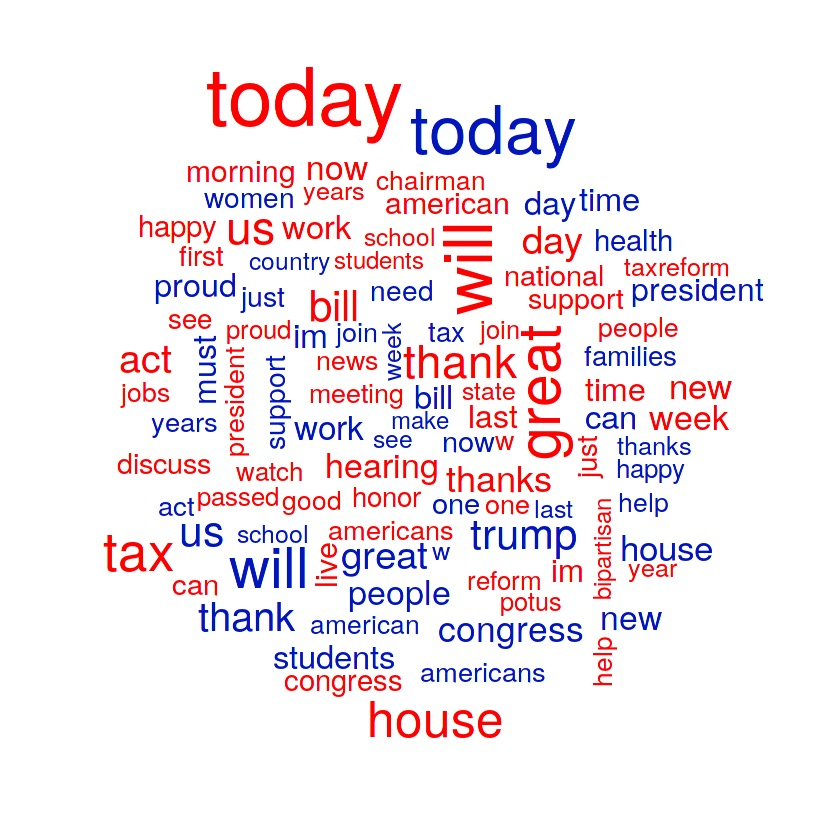
\includegraphics[width=0.25\textwidth]{proposal-latex/figures/top100.jpg}
    \caption{Top 100 words in the data set \cite{nnnnick_2018}}
    \label{fig:top100}
\end{figure}

\subsection{Computational Tools}
The computer hardware will be group team members' laptops, and the computation might be performed on the remote/cloud platform. The computational software that will potentially be used in this project are Python, Jupyter notebook, Numpy, Scikit-Learn, and some other packages. 

\section{Contributions}

For the computational task of the project, Han will be responsible for data prepossessing, researching and implementing a machine learning pipeline, Siyi will be responsible for developing and tuning the models, and Qiwen will be responsible for evaluating the model. For the report writing task, Han will be responsible for the introduction and the overall organization of the report, Siyi will be responsible for the methods of the model and related work, and Qiwen will be responsible for results and conclusion.

{\small
\bibliographystyle{ieeetr}
\bibliography{bibliography.bib}
}

\end{document}
